\chapter{INTERFACE IMPLEMENTATION}
\label{chap:GUI_impl.tex}
\section{INTERFACE}
The necessity to enhance manual debug methodology has been established in \sectionname{\ref{sec:enhancement.tex.nemv}} and certain requirements of such an interface is established in \sectionname{\ref{sec:enhancement.tex.emv}}. This chapter concentrates on design and implementation of the debug interface.

The debug interface is aimed at being intuitive and user friendly. It should aid data navigation so as to reduce manual efforts. If user requires to refer to actual processor execution log or assembly code, it should be readily availalbe through the interface. The interface should also provide graphical representation of processor execution log, to aid traversal and filtering of processor activity. The interface should aid traversing through processor execution easy.  Critical events made by processor should be extracted, categorized and made availabe to user.

In addition to interface requirements listed in \sectionname{\ref{sec:enhancement.tex.emv}}, the following set of features would also aid in debug:

\begin{itemize}
\item[-] Visualizing thread-wise execution flow
\item[-] Ability to highlight instances of critical activities such as Memory write/read, I/O write/read, Branching etc
\item[-] Interrupt and exception happening during execution
\item[-] Assembly code traversal and its linkage with execution flow
\item[-] Register current state value traversal and its linkage with execution flow
\item[-] Comparison of register values between arbitrary instances of execution
\item[-] Simulation cycle of execution event
\end{itemize}

Every stimulus is a unique assembly test and hence the debug interface should be as generic as possible. It should be able to accomodate any relevant assembly test, accompanied with execution logs.

%Once the simulation is completed and failure is reported the debug phase starts. This is where the role of GUI comes. From the vast information provided by the logs and test files, interfaces have to capture and represent relevant information to the user. The following section details the implementation and features of the proposed GUI. 

\subsection {CHOOSING GUI}
There are multitude of languages providing GUI capability, the project doesnot need a very sophisticated GUI implementation. Moreover the interface should aid remote debug and if possible thee should not be any requirement for any user to install a tool-kit or library for the debug interface to be used. Hence the decision to use web-browser as the debug interface was a default choice. A web browser could also execute {\it javascripts} and that makes it customisable. The design is also scalable and aids introduction of new features for debug with ease.

Each stimulus will have its own set of assembly test files and execution log files. The interfaces implementation starts by consuming these files. Two programming languages are used for implementation:
\begin{description}
\item[Python Script] for data extraction and correlating related information.
\item[JavaScript] for designing the interface features and user interaction.
\end{description}

\addtocontents{toc}{\protect\setcounter{tocdepth}{2}}
%\figurename{} 
\begin{figure}[h]
\centering
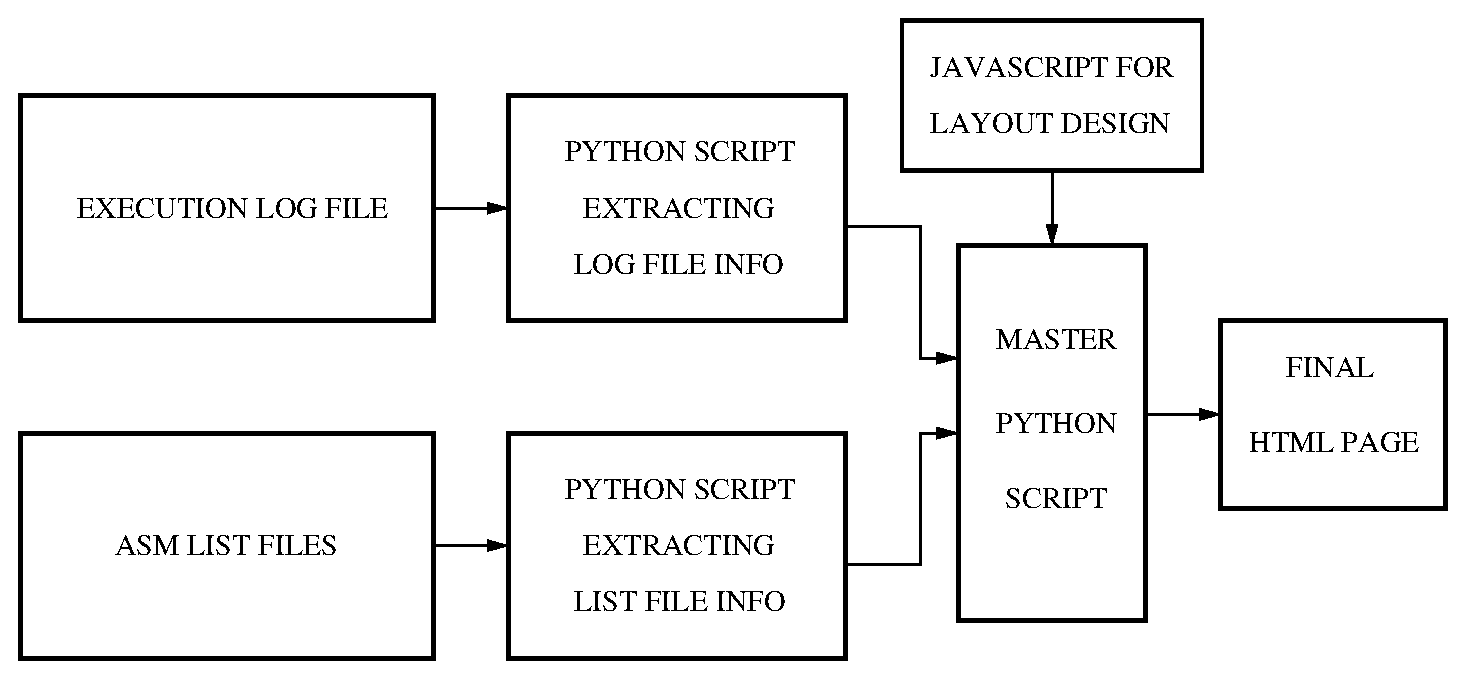
\includegraphics[width=5.5in]{./figures/gui_impl.eps}
\caption{GUI Implementation} 
\label{fig:gui_impl.eps}
\end{figure}

\figurename{\ref{fig:gui_impl.eps}} depicts information extraction and use of different scripts to achieve the same. Major implementation steps
\begin{itemize}
\item[-] Extraction of information from assembly list file and processor execution log by python script.
\item[-] Correlation of information from previous step.
\item[-] Coding generic JavaScript code for user interactions.
\item[-] Top level python program to manipulate available information and to convert it to JavaScript information. 
\item[-] The top level python program will combine the data extracted and javascriot code to generate a single HTML page. 
\end{itemize}

The whole infrastructure is packaged neatly. Given execution log file and assembly list file, the top level python script generates the HTML interface web page. Different stages involved in this conversions are described in the following sections. 

\subsection {INTERFACE}
GUI is targetted to run on any browser, hence layout design is done using {\it HTML}\nomenclature{HTML}{Hyper Text Markup Language}. However for providing interactive features to the user, a much more powerful language is need along with HTML and default choice is JavaScript.

\emph {\bf JavaScript (JS)} is an interpreted computer programming language. It is  implemented as part of web browsers so that client-side scripts could react to user inputs, customize the browser, communicate asynchronously, and to filter contents being displayed. It is a multi-paradigm language, supporting object-oriented, imperative, and functional programming styles.  
In addition a style sheet language called CSS\nomenclature{CSS}{Cascading Style Sheets} is used for describing the presentation semantics (the look and formatting) of the interface page written in HTML.

%\figurename{} 
%\figurename{} 
\begin{figure}[h]
\centering
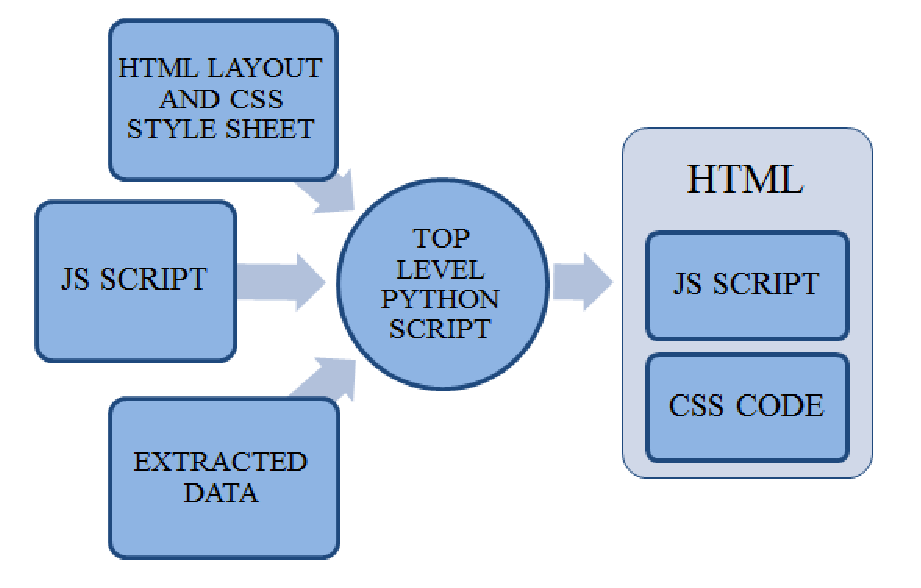
\includegraphics[width=3.5in]{./figures/html.ps}
\caption{Web Page Generation}
\label{fig:impl:wpg}
\end{figure}

Resultant HTML page embeds JavaScript routines and style sheets. This is done by the top level python script. \figurename{\ref{fig:impl:wgp}} shows a representation of information flow.


\subsection{JS DATASTRUCTURE}
All dynamic features of the interface are handled by JS\nomenclature{JS}{JavaScript} script routines. Data input to the JS is the extracted information from execution log files and list files. The top level python script converts the extracted objects into JS data array ``$dataArray[]$'' ; where each array element coresponds to an active thread. Active threads refer to active core or processor in a multiprocessor system.  

\IncMargin{1em}
\begin{algorithm}[h]
\DontPrintSemicolon
\SetKwInOut{Input}{Input}\SetKwInOut{Output}{Output} \SetKwFunction{KwFn}{CreateDataArray}
\KwFn {}
\BlankLine
\Begin{
\For {i in activeThreads}{\;
		\For {$log$ in logObj}{\;
		\If{log.Id == i}{
		Append $log \rightarrow	DataArray[i]$\;
		}
}
}
}
\caption{Creating JavaScript Object}
\end{algorithm}\DecMargin{1em}



Once the extracted information is converted to JS compatiable data, the interface features can utilize this. The layout for various GUI features called windows, are designed using HTML and CSS code. All dynamic interactive featurers are handled by embedded JS script in HTML web page. Later sections introduces different windows availabe in the web page.

\section {EXTRACTION OF INFORMATION}
The first step in creating a generic debug interface is to extract relevant information and convert it to a format that could be loaded by the debug interface.

\subsection {STIMULUS}
Stimulus is written in X-86 assembly language. The engineer is expected to debug this stimulus. Each cycle in processor execution log corresponds to a particular assembly code. An assembler is used to assemble to object code, in that process each instruction is also mapped to a particular address. \figurename{\ref{impl.tex:assembler}} shows this process which also produces a list file which hold an macro expanded, loop unrolled, assembled code with corresponding address details. The configuration file defines certain random operands, segmentation, gdt, ldt, page tables to aid in assembling process. The include files contribute common routines used across different assembly stimuluses.

%However, the written by the verification engineer is the unscheduled code without any memory address details. For cycle comparison with execution log, the asm test file is complied first.

\begin{figure}[h]
\centering
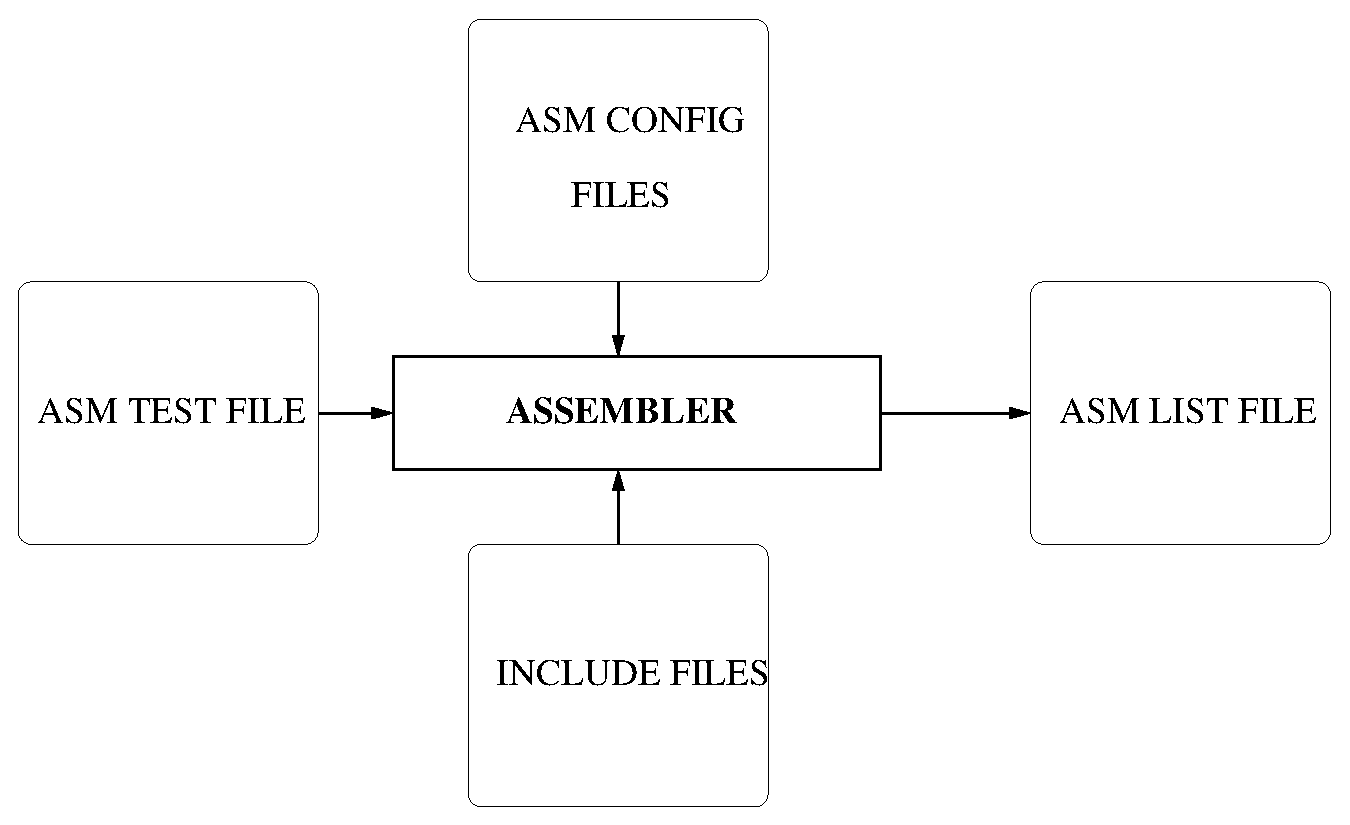
\includegraphics[width=3.5in]{./figures/asm.ps}
\caption{Assembler}
\label{impl.tex:assembler}
\end{figure}


\begin{figure}[h]
\centering
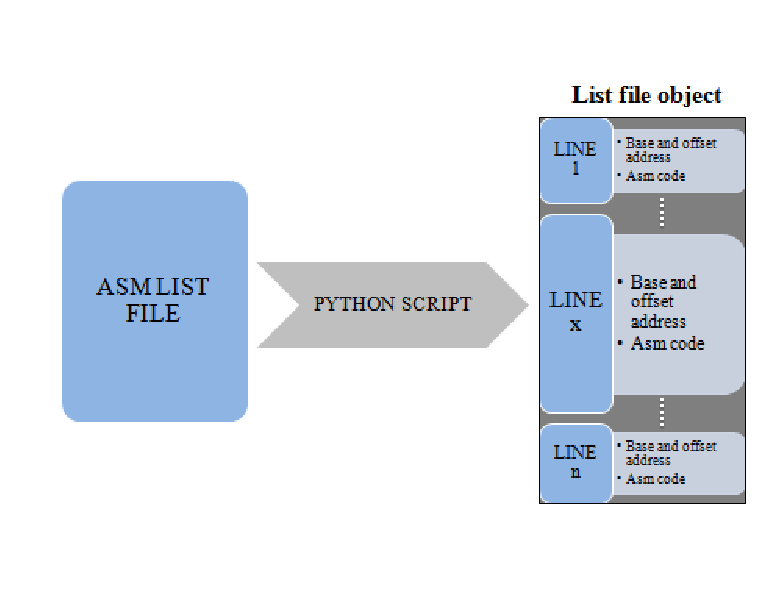
\includegraphics[width=4.5in]{./figures/list.ps}
\caption{Asm List File Extraction}
\label{impl.tex:listextr}
\end{figure}

List file holds a wealth of details including instructions, opcodes, operand, linear address, module/register configuration details etc. A {\it python} script is used to extract relevant information corresponding to each instruction line in the list file. In this project, the following information is extracted for each instruction from the  list file:
\begin{itemize}
	\item[-] Base and offset address value
	\item[-] Instruction line number
	\item[-] The assembly code
\end{itemize}

The {\it python} script internally contains a data structure of list objects, which helps in adding features to the script with ease (\figurename{\ref{impl.tex:listextr}}). 

\subsection {EXECUTION LOG}
Execution log file contains instruction by instruction execution details from simulation. It also includes register states, thread details, flag values and other details which help in tracing out the cause of failure. As explained in previous chapters, debugging require detail traversal through this log file. 

Details in the log file with reference to each cycle is required to be extracted. {\it Python} script is used to extract these informations as well and a comprehensive data structure is created. The data structure objects contain properties corresponding to major operations and register values. Thread details are handled as seperate data structures as it aids processing thread-wise informations. Following properties are extracted from execution log file for every execution event

%Figure x shows how the script will read the input execution log file and generate log file objects.

\begin{itemize}
 \item[-]  Thread number
 \item[-]  Mode of operation
 \item[-]  Cycle number
 \item[-]  Linear address
 \item[-]  Memory write, Memory read, I/O write/read, Code read
 \item[-]  Branch target (linear address)
 \item[-]  New values of registers, if modified
\end{itemize}


\subsection {INFORMATION CORRELATION}

Once both the input files are processed, next step is to correlate assembly with execution log. A {\it python} script can accompish this by correlating respective data structures based on linear addresses. As x86 architecture follows segmented memory model along with paging, address translation is required for generating the linear/physical address\cite{SS:AMD64-V2}. Linear address is calculated as
\\
\centerline{Linear address = Base address + Offset value}
\\


%\vspace{1.5cm}

\IncMargin{1em}
\begin{algorithm}[h]
\DontPrintSemicolon
\SetKwInOut{Input}{Input}\SetKwInOut{Output}{Output} \SetKwFunction{KwFn}{CreateDataArray}

\Input{list file objects$\rightarrow listObj[]$, log file object$\rightarrow logObj[]$}
\BlankLine
Start: \;
\For {each object $list$ in listObj}{\;
		list.address = list.Base + list.Offset\;
	}
\For {each object $log$ in logObj}{\;
	set count = 0\;
	\For {each object $list$ in listObj}{\;
	 \If{$log.address == list.address$}{
		Append each $list$.property $\rightarrow$ $log$.property\; \tcp{$log$ properties are lineNo, opcode and address}\label{cmt}
		count = 1;
		break loop\;
	}
	}
	\If{count == 0}{
	assert: $"no address match"$
	}
}
End \;
\caption{Combining List and Log File Information}
\label{algo:impl:cllf}
\end{algorithm}\DecMargin{1em}

%\vspace{1.5cm}

For each object of execution log, the corresponding list file object could be found based on linear address value. Once found, both are cross-linked to aid further processing. The alogorithm employed in this search is depicted in Algorithm~\ref{algo:impl:cllf}. Data extraction is complete with this linkage and the result is execution log objects linked to corresponding assembly objects.

\section {GUI FEATURES}

\subsection {EXECUTION FLOW GRAPH}
Main feature of debug interface is the graph showing the execution flow of the code. It is obtained by plotting asm list file line numbers against the execution cycle during which it is executed. All the active threads have different graphs which are tabbed. Hovering the mouse over any execution point on the graph will display $X$ and $Y$ axis values. Features include zoom-in, zoom-out of plot. Double click at any point is featured to zoom-out completely. On clicking on any execution point, selects the point and sychronises data across windows. Proximity click feature helps in automatically choosing nearest execution point for further analysis.
 
The flow graph also features customisable selection of specific processor operations out of Branching, Memory Write, Memory Read, Code Read. This helps in filtering redundant execution points those may not be of interest to the engineer. Each distinct processor operation could be distinguished by color coding.   

\subsubsection {IMPLEMENTATION}

Execution flow graph is created with Dygraph JavaScript Visualization Library\cite{http:dygraphs}. The library provides inbuilt functions that enable zooming, x-y axis value display and point ``{\it onClick}'' callbacks. {\it onClick CallBack()} function is called whenever an execution point on Dygraph is clicked. The function has been extended to activate other windows and to synchronize components across windows.

Graph could be built by providing independent axis values followed by depended axis values. For each thread, a different graph is generated but layered out on different HTML tabs. The x-axis is cycle number and y-axis is the list file line number. Algorithm~\ref{algo:impl:ceg} shows the pseudo-code used in building the graph in our application.

\IncMargin{1em}
\begin{algorithm}[h]
\DontPrintSemicolon
\SetKwInOut{Input}{Input}\SetKwInOut{Output}{Output} \SetKwFunction{KwFn}{CreateGraph}
\KwFn{}
\BlankLine
\Begin{
\For {each i in activeThread}{\;
\For {each element in dataArray[i]}{\;
	Dygraph[i] $\leftarrow [element.cycleNo , element.lineNo]$\;
	}
}
}
\caption{Creating Execution Graph}
\label{algo:impl:ceg}
\end{algorithm}\DecMargin{1em}

\subsection {REGISTER WATCH WINDOW}
\label{sec:impl:rww}
Register window is used in displaying instantaneous register values at any execution point. Under the hood, thread based register values are maintained seperately, as it aids user switching back and forth between threads of execution without loosing data on each thread. At any instant the register window holds the values of {\it selected} execution point. Selection could be changed by simply clicking on a different execution point. Register window provides values of following registers to the user:
\begin{itemize}
	\item[-] 64 bit general purpose registers (RAX, RBX, RCX etc)
	\item[-] RFLAG (64 bit)
	\item[-] Instruction Pointer (RIP)
	\item[-] Stack Pointer (RSP)
\end{itemize}

Another important feature provided by register window is a comparision of register values between two different execution points. It highlights differences in register values with different colours, to capture user's attention with ease. The diff is between {\it reference execution point} and {\selected execution point}. {\it Reference execution point} is choosen by the {\it set~marker} button.

\subsubsection{IMPLEMENTATION}

The values contained in register window is updated when a different execution point is selected in the execution flow graph. This event also trigges there comparison of current values with the reference point. Algorithm~\ref{algo:impl:crw} lists the pseudo-code used in updating register window values.

\IncMargin{1em}
\begin{algorithm}[h]
\DontPrintSemicolon
\SetKwInOut{Input}{Input}\SetKwInOut{Output}{Output} \SetKwFunction{KwFn}{pointonClickCallBack}
\KwFn{element}
\BlankLine
\Begin{
\For {each reg in RegisterSet}{
regRow$[reg]$ $\leftarrow$ element.$[reg]$ \;
	\If{(element.$[reg]$ != referenceRow.$[reg]$)}{\;
		$Highlight  regRow $ \;
	}
}
}
\caption{Creating Register Window}
\label{algo:impl:crw}
\end{algorithm}\DecMargin{1em}

\subsection {INSTRUCTION WINDOW}

Instruction window lists the assembly code corresponding to the selected execution point. Context around the assembly code is also displayed to aid debug. This window is also updated when a different execution point is selected in execution graph. The window highlights assembly code for visual attention of the user.

\subsubsection{IMPLEMENTATION}

The pseudo-code used to update values in this window is shown in Algorithm~\ref{algo:impl:ciel}.

\IncMargin{1em}
\begin{algorithm}[h]
\DontPrintSemicolon
\SetKwInOut{Input}{Input}\SetKwInOut{Output}{Output} \SetKwFunction{KwFn}{onClickCallBack}
\KwFn{element}{;\
\BlankLine
\Begin{
\For {each item from elemnt-50 to element+50}{\;
	Add $item.opcode \rightarrow$ InstructionWindow\;
	}

Add $item.logInfo \rightarrow$ ExecutionLogWindow\;
}
}
\caption{Creating Instruction and Execution Log Window}
\label{algo:impl:ciel}
\end{algorithm}\DecMargin{1em}

\subsection {EXECUTION LOG WINDOW}

In addition to the instruction and register information, the relevant processor execution log in its actuality would be useful to the user as it contains different information that may not be presented by the debug interface. Having this information readily accessable to user also assures the user that the data extracted through processing by different scripts is indeed correct. Internally these informations are stored as a JavaScript object "{\emph logInfo}". 

%Implementation of Execution log window is given in algorithm x along with instruction window.

\subsection{MARKERS}
As it was discussed in \sectionname{\ref{sec:impl:rww}}, markers are used to ``mark'' reference execution point through a ``Set Marker'' button. Button ``Clear Marker'' could  be used to clear the marker.

\subsubsection{IMPLEMENTATION}

Set and Clear buttons are implemented using HTML form's callback feature. A {\it JavaScript} variable is used to store the reference execution point.


